%%%%%%%%%%%%%%%%%%%%%%%%%%%%%%%%%%%%%%%%%%%%%%%%%%%%%%%%%%%
% --------------------------------------------------------
% Tau
% LaTeX Template
% Version 2.4.3 (01/09/2024)
%
% Author: 
% Guillermo Jimenez (memo.notess1@gmail.com)
% 
% License:
% Creative Commons CC BY 4.0
% --------------------------------------------------------
%%%%%%%%%%%%%%%%%%%%%%%%%%%%%%%%%%%%%%%%%%%%%%%%%%%%%%%%%%%

\documentclass[9pt,a4paper,twoside]{tau-class/tau}
\usepackage[english]{babel}
\usepackage[most]{tcolorbox}
%----------------------------------------------------------
% TITLE
%----------------------------------------------------------

\journalname{Fundamentals of Natural Language Processing}
%% TODO: Optional, you can set a fancier title if you like
\title{Negation and Uncertainty Detection using Classical and Machine Learning Techniques}

%----------------------------------------------------------
% AUTHORS, AFFILIATIONS AND PROFESSOR
%----------------------------------------------------------

%% TODO: Set your names here
\author[a]{Tomàs Ockier Poblet}
\author[b]{Yaira Brudenell Guedella}
\author[c]{Gerzon Díaz Marcani}
\author[d]{Samuel Fontdecaba Pérez}

%----------------------------------------------------------

\affil[a]{1707185}
\affil[b]{1707353}
\affil[c]{1704153}
\affil[d]{1706954}

%----------------------------------------------------------
% FOOTER INFORMATION
%----------------------------------------------------------

\institution{Universitat Autònoma de Barcelona}
\footinfo{NLP Project}
\theday{\today}
\leadauthor{Group 9} 		%% TODO: Set your group ID here
\course{Fundamentals of Natural Language Processing}

%----------------------------------------------------------
% ABSTRACT AND KEYWORDS
%----------------------------------------------------------

\begin{abstract} 
	%% Keep it below 300 words
    We present a rule-based method for detecting negation and uncertainty cues, as well as their scopes, in clinical Spanish and Catalan texts. By leveraging a lexicon of predefined linguistic cues, our approach systematically segments the text into sentences, enabling identification of negation and uncertainty patterns. Our prototype can be used as a baseline in order to create more complex models with Machine Learning and Deep Learning methods.
\end{abstract}

%----------------------------------------------------------

%%
\keywords{Negation detection, Uncertainty detection, Clinical text analysis, Rule-based approach, ML}

%----------------------------------------------------------

\begin{document}
	%% Do NOT change any of this. Line numbers should be kept. 
    \maketitle 
    \thispagestyle{firststyle} \tauabstract 
    \tableofcontents
    \linenumbers 
    
%----------------------------------------------------------

\section{Introduction}

    \taustart{M}any details in medical records are written in an unstructured way, often as notes or summaries, making them hard for both automated systems and humans to fully access for clinical or research use. While information retrieval tools can help search these texts, they often fail to distinguish between terms that are affirmed, negated, or uncertain. Negation words are usually treated as stop words and ignored, which leads to misleading results.
    
    The presence of a medical term in a report does not necessarily imply the patient has the condition. It may be explicitly denied or mentioned with uncertainty. These expressions in clinical notes and are crucial for accurate understanding. Identifying not just the negation, but also the uncertainty, and determining which terms are actually affected is essential for meaningful indexing and analysis.
    
    Although some medical language processing (MLP) systems can handle negation and uncertainty, they are often not easily reusable. In this project, we present and test a simple algorithm using basic rules to detect negation, uncertainty; and their scope, helping to better process and index narrative clinical data.

% quizás podemos quitar esto, o fusionar parte de esta info en la intro (?)
\section{Exploratory Data Analysis}

	For the first part of the project we had to explore the data to understand it to be able to handle it better for our goal. We extracted and transformed the data into a \textit{DataFrame} so that it was more manageable. 
    There are four labels, \textit{NEG} and \textit{UNC} for the cues of negation and uncertainty and \textit{NSCO} and \textit{USCO} for their respective scopes, if any. 
    There are considerably more negation sentences than uncertainty ones, as we can see in Fig. \ref{fig:distribution-labels}.
    
    \begin{figure}[H]
        \centering
        \includegraphics[width=0.7\linewidth]{nlp/figures/label_distribution.pdf}
        \caption{Distribution of label types}
        \label{fig:distribution-labels}
    \end{figure}
    

\section{Preprocessing} \label{sec:prep}
    % \subsection{Libraries and Tools Used}
    % Several libraries were employed in our project. Below is a summary of them and their functions:
    % \begin{itemize}
    %     \item \textbf{NLTK}: Used for various natural language processing tasks. Specifically, the \lstinline|TreebankWordTokenizer| was used to tokenize text, and standard tokenization utilities like \lstinline|word_tokenize| supported word-level segmentation.
        
    %     \item \textbf{pandas}: Used for handling structured data, particularly annotation tables in CSV format. 
                
    %     \item \textbf{pickle}: Used to serialize processed annotation dataframes (e.g. \lstinline|df_train.pkl|), avoiding the need to reprocess raw inputs.

    %     \item \textbf{sklearn\_crfsuite}: used to train and evaluate the CRF model. It models the conditional probability of label sequences given input sequences, using handcrafted features. It supports various optimization algorithms and integrates well with scikit-learn tools.

    %     \item \textbf{sklearn}: for model selection through \texttt{GridSearchCV} to find hyperparameters that yields the highest model performance on validation data.
        
    % \end{itemize}

    \subsection{Preprocessing of Data}
    The preprocessing pipeline employs an \lstinline|AnnotationProcessor| class designed to structure unstructured text for the annotation tasks. This component performs two core operations: (1) line segmentation via a tokenizer and (2) token span mapping with positional indexing.

        \begin{tcolorbox}[colback=blue!20, colframe=blue!20, sharp corners, boxrule=0.5pt]
        \subsubsection*{Annotation Pipeline (formal representation of the process)}
        The \lstinline|process_data| method coordinates the preprocessing workflow by:
        \begin{enumerate}
        \item Generating line-segmented text files with character offset indexes
        \item Projecting character annotations to token positions:
        
        \begin{equation}
            \tau_i = \underset{\tau \in \mathcal{T}}{\arg\min} \left( \delta_{start}(\tau) \leq \alpha_c \leq \delta_{end}(\tau) \right)
        \end{equation}
        
        where $\alpha_c$ denotes annotation character offset and $\delta$ represents token span boundaries.
        \end{enumerate}
        \end{tcolorbox}
        
        After the mapping, the processed annotations are stored DataFrames for train and test. Each row corresponds to an annotated span and contains the following fields: \texttt{doc\_id} (document identifier), \texttt{line\_id} (line number in the document), \texttt{annotation\_id} (unique ID for the annotation), \texttt{start} and \texttt{end} (token-level span indices), \texttt{label} (e.g., NEG, NSCO), and \texttt{text} (the annotated span content).
    
\section{Rule-Based Approach} \label{sec:rule-based}

    \subsection{Overview}
        This approach relies on lexical pattern matching, without using machine learning, focusing on explicit linguistic cues that signal negative assertions or uncertain statements in clinical documentation. This approach creates predictions based only on text pattern matching, without using existing labels.

    \subsection{Lexicon}
        The system relies on two primary resources: 
        \begin{enumerate}
            \item \textbf{Negation Lexicon}: Contains terms indicating absence or denial (e.g., "no", "sin", "negativo") 
            \item \textbf{Uncertainty Lexicon}: Contains terms indicating possibility or doubt (e.g., "puede", "compatible con", "descartar")
        \end{enumerate}
        
        Both contain catalan and spanish cues, mostly related to the medical domain, but as we know, in these languages, the morphological variations are common. We aim at catching the different ways in which a cue can present, with variations in number and gender of the word.

        
    \subsection{Methodology}
        \subsubsection{Cue Detection}
        After the medical documents are preprocessed, each tokenized line passes through a function to find its negation cues. It does so by comparing every different word in the lexicon with the token by \textbf{exact matching}. When a match is found, the system records in a dictionary useful information related to the indexes, the ID of the document and the line, and both the token and the "canonical" term it had supposedly matched. It first checks for negation and then for uncertainty since it works the same for both.

        \subsubsection{Scope Determination}
            Once cues are identified, determining their scope of influence is a more complex task that involves four different rules based on cue type:        
        \begin{enumerate}
            \item \textbf{Standard Negation Cues:} It is divided into a Forward and a Backward Scope Rule. The scope typically extends from the cue end to the next punctuation mark. But if the punctuation follows the cue, the scope may affect preceding text.
            
            \item \textbf{Negative Adjectives:} It uses similar scope rules but potentially different contextual effects. In medical texts, these often modify preceding noun phrases. This helps capture phenomena like "fiebre: negativo".
            
            \item \textbf{Verbal Negation:} More focused scope, usually affecting the noun or noun phrase immediately after it. But if no punctuation mark is found, the end of the scope is set as the end of the text, because terms like "niega" typically precede a list of symptoms being denied. Again, in the case where the cue immediately follows a punctuation mark, it defines the scope backwards.
            
            \item \textbf{Uncertainty:} It is a simple rule since the scope typically extends from the uncertainty cue to the next punctuation mark.
        \end{enumerate}

        Periods, commas, semicolons, and colons act as scope terminators. And for each detected scope, we store the useful information in our prediction dictionary as we previously did with the cues. 

    \subsection{Evaluation}
        Once both cues and their scopes are determined, the system creates structured annotations with the correct format to evaluate the performance. The total count of labels is very close to the actual one, and the distribution is somewhat close too, as we can see in Table \ref{fig:label_counts}. 
        \newline
        \begin{table}[h!]
            \centering     
            \begin{tabular}{|l|c|c|} % que no os dé pena borrar esto si no lo queremos
            \hline
            \centering
            Label & True & Pred. \\ \hline
            NEG & 4307 & 4503 \\ \hline
            NSCO & 4103 & 3682 \\ \hline
            UNC & 458 & 563 \\ \hline
            USCO & 451 & 321 \\ \hline
            \end{tabular}
            \caption{Comparison of label counts}
        \label{fig:label_counts}
        \end{table}

        We calculated the overall entity matching accuracy, using the \textbf{Jaccard Index method}, which, unlike the traditional accuracy, takes into account the false negatives in the denominator so it makes it less optimistic and more realistic, and it got a 42,47\%. But then, we computed it again only considering the results of the cues, and it raised to a 75.62\%, suggesting that the model struggles with the scopes. This is because an exact match requires identical \lstinline|line_number|, \lstinline|start|, \lstinline|end|, and \lstinline|label|. This supports the hypothesis that partial matches are penalized too harshly with this metric. For example, in some scopes, the "." is included too and it makes the entire span to be counted as wrong. This is why we made it less restrictive by tokenizing or splitting the annotations into new ones (preserving its correct index and label). Now, with this expanded version of the annotations, the accuracy increased to 58.04\%, as we expected.
        \newline
        
        \begin{figure}[H]
            \centering
            \includegraphics[width=0.85\linewidth]{nlp/figures/confusion_matrix_eval.png}
            \caption{Confusion Matrix made with the predictions on the training data}
            \label{fig:confusion_matrix_eval}
        \end{figure} 

        Finally, we measured the errors with this expanded version of the predictions. In figure \ref{fig:confusion_matrix_eval} we can see a confusion matrix where the rows represent true labels and columns represent predicted labels. The values on the diagonal are the true positives. The special column 'FN' represents missed predictions (omissions) and the 'Null' row represents non-entity states (background text, or mistakes).

        By analyzing in which cues errors were made, it can be observed that the majority are for "sin" and "no", which are the cues that are most presented on the train data.
        
        The final results presented were achieved after looking at the errors and performing statistical analysis to detect the most common ones. We removed the keywords that result in more false positives than true negatives. As in the beginning the list of the keywords that triggered the scope detection was quite large. We believe that with more care the scope detection could be improved.

        Developing a Machine Learning model could result on better results, as we believe that it would allow us to distinguish better between the "sin" and "no" examples in the dataset. They result on the great majority of false positives for the NEG and NSCO. The same can be said of "puede" for UNC and USCO.

        \subsubsection{Evaluation on Test Dataset}
        The same type of evaluation was performed on the test dataset that was provided. The test data was not the basis of any of the rules or lexicon creation that formed part of our model.

        We found the same results on the test data, with an overall accuracy of 58.73\%, using the individual token evaluation. Just taking into account the NEG and UNC labels, 75.20\%. The same types of errors were found, with a prevalence of false positives for "no" and "sin".

        These metrics seem to indicate that the test and training data are extremely similar.

\section{ML Approach - CRF's} \label{sec:ML-based}
      \subsection{Overview}
        Conditional Random Fields (CRFs) are a type of probabilistic model that define a conditional distribution over possible label sequences given an input sequence. This allows the model to focus on the structure of the output without making important assumptions about the input.
        \\
        Unlike the rule-based method, CRFs use contextual features and dependencies between neighboring labels, which allows for better generalization to unseen or ambiguous cases of uncertainty and negation.
        
        \subsection{Preprocessing}
        To prepare the training data for the CRF model, we implemented a function that aligns each token with its corresponding annotation label. This function, \lstinline|data_to_tagging|, processes each clinical document previously split line by line. Using the same tokenizer as in the preprocessing, it splits the lines into tokens. It also takes the dataframe containing annotated spans (with start and end indices) and labels. See \nameref{sec:prep} for more details about the preprocessing steps.
        Tokens are initialized with the label O ("Other"). For each annotated line, the corresponding token spans are updated with the proper tag. The function returns two dictionaries:
        \begin{enumerate}
            \item One mapping line IDs to token sequences.
            \item Another mapping line IDs to their respective tag sequences.
        \end{enumerate}
        
        This output serves as the input for the CRF, where each token is paired with its tag for supervised learning.

        
    \subsection{Methodology}
        \subsubsection{Feature Extraction}
        For each token, we generate the following features to train the CRF model, these aim to capture the characteristics of the token and its local context:

\textbf{Token-level features:}
    \begin{itemize}
        \item \texttt{word}: The token itself.
        \item \texttt{lower}: Lowercase version, useful for normalization.
        \item \texttt{is\_upper}: Boolean flag for all-uppercase tokens (e.g., acronyms).
        \item \texttt{is\_title}: Indicates if the token is capitalized.
        \item \texttt{is\_digit}: Flags numeric tokens (e.g., dates).
    \end{itemize}
    
    \textbf{Contextual features:}
    \begin{itemize}
        \item \texttt{-1:word}: Lowercase form of the previous token (if it exists).
        \item \texttt{+1:word}: Lowercase form of the next token (if it exists).
        \item \texttt{BOS}: True if the token is at the beginning of a sentence.
        \item \texttt{EOS}: True if the token is at the end.
    \end{itemize}


        \subsubsection{Model Training}
            We employed two different optimization algorithms for training: L-BFGS and L2SGD.
            \begin{enumerate}
                \item \textbf{L-BFGS} is a second-order optimization method that uses both the gradient and an approximation of the second derivatives (Hessian matrix) to optimize the model. It provides faster convergence and more stable optimization and uses both L1 and L2 regularization. L-BFGS tends to outperform other methods in terms of accuracy and convergence for moderate-sized datasets.
                
                \item \textbf{L2SGD} is a first-order optimization algorithm. It only considers the gradient and uses L2 regularization, making it more memory-efficient and faster, but it may take longer to converge and can be less stable than L-BFGS.
            \end{enumerate}

        Both algorithms were tuned using GridSearchCV to optimize hyperparameters such as regularization strength and maximum iterations. 
        \begin{table}[h]
        \centering
        \begin{tabular}{|l|l|}
        \hline
        \textbf{Algorithm} & \textbf{Best Parameters} \\
        \hline
        \texttt{lbfgs} & \{c1: 0.1, c2: 0.1, max\_iterations: 50\} \\
        \texttt{l2sgd} & \{c2: 0.1, max\_iterations: 50\} \\
        \hline
        \end{tabular}
        \caption{Best hyperparameters found for each CRF optimization algorithm using Grid Search}
        \end{table}


    \subsection{Evaluation}
        The goal was to find the best performing algorithm for the dataset by evaluating their performance based on cross-validated accuracy. 

        \begin{table}[h]
        \centering
        \caption{Classification report for CRF model with LBFGS algorithm}
        \begin{tabular}{|l|c|c|c|c|}
        \hline
        \textbf{Label} & \textbf{Precision} & \textbf{Recall} & \textbf{F1-Score} & \textbf{Support} \\
        \hline
        NEG   & 0.973 & 0.929 & 0.951 & 1181 \\
        UNC   & 0.937 & 0.604 & 0.735 & 197  \\
        NSCO  & 0.919 & 0.817 & 0.865 & 3550 \\
        USCO  & 0.892 & 0.615 & 0.728 & 564  \\
        \hline
        \textbf{Micro Avg}    & 0.930 & 0.813 & 0.867 & 5492 \\
        \textbf{Macro Avg}    & 0.930 & 0.741 & 0.820 & 5492 \\
        \textbf{Weighted Avg} & 0.928 & 0.813 & 0.865 & 5492 \\
        \hline
        \end{tabular}
        \end{table}
      
        \begin{table}[h]
        \centering
        \caption{Classification report for the CRF model using L2SGD algorithm}
        \begin{tabular}{|l|c|c|c|c|}
        \hline
        \textbf{Label} & \textbf{Precision} & \textbf{Recall} & \textbf{F1-Score} & \textbf{Support} \\
        \hline
        NEG   & 0.975 & 0.924 & 0.949 & 1181 \\
        UNC   & 0.943 & 0.503 & 0.656 & 197  \\
        NSCO  & 0.944 & 0.789 & 0.860 & 3550 \\
        USCO  & 0.886 & 0.441 & 0.589 & 564  \\
        \hline
        \textbf{Micro Avg}    & 0.948 & 0.772 & 0.851 & 5492 \\
        \textbf{Macro Avg}    & 0.937 & 0.664 & 0.763 & 5492 \\
        \textbf{Weighted Avg} & 0.945 & 0.772 & 0.844 & 5492 \\
        \hline
        \end{tabular}
        \end{table}

        \begin{figure}[H]
            \centering
            \includegraphics[width=0.85\linewidth]{nlp/figures/cmatrices.png}
            \label{fig:confusion_matrix_eval}
            \caption{Confusion Matrix Results for the CRF model}
        \end{figure} 
        
    \subsection{Results}
        UNC (Uncertain scope) is the most challenging class for both models. However, L-BFGS outperforms L2SGD, particularly in USCO and UNC, which are more context-sensitive.

        Both models outperform the rule-base method and L-BFGS is preferred due to higher accuracy in the harder-to-predict classes and a better balance between precision and recall. It's computationally more expensive but more stable for this task. 

\section{ML Approach - HMM} \label{sec:hmm-based}
    \subsection{Overview}
        Hidden Markov Models (HMMs) are statistical sequence models where each token's label only depends on the previous token's label (Markov property). We thought this limitation might cause HMMs to struggle with negation and uncertainty detection, since these usually need understanding of longer dependencies. Also, because of the chain rule, we expected errors to spread when one token is wrong, the next ones are likely to be wrong too. Even with these challenges, we still wanted to try HMMs to get a statistical baseline and see if we could make improvements to overcome these limitations.
    \subsection{Methodology}
        For our models, hidden states are the labels (NEG, NSCO, UNC, USCO, O) and observations are the tokens. We tried three different versions, each one more complex than the last.
        
        \begin{enumerate}
            \item \textbf{Baseline HMM}. Just uses word tokens as observations, learning emission probabilities $P(word|label)$ and transition probabilities $P(label_t|label_{t-1})$.
            
            \item \textbf{BIO+POS HMM}. Adds two improvements. First, BIO tagging to better find entity boundaries. Second, Part-of-Speech features combined with tokens to get richer observations.
            
            \item \textbf{Second-Order HMM}. Goes one step further by looking at two previous states $P(label_t|label_{t-1},label_{t-2})$, trying to fix the limited dependency window.
        \end{enumerate}
        
        We trained all models with Laplace smoothing (parameter=0.01) and used Viterbi for inference.
    \subsection{Results}
        Figure \ref{fig:hmm-comparison} shows how the different models performed. The baseline got an F1 score of 0.56, then the BIO+POS model jumped to 0.73 (a 30.4% increase). Our second-order model reached 0.78, another 6.8% gain. These results suggest that even though HMMs have theoretical problems for this task, our enhancements really helped overcome some of these issues.
        
        \begin{figure}[H]
            \centering
            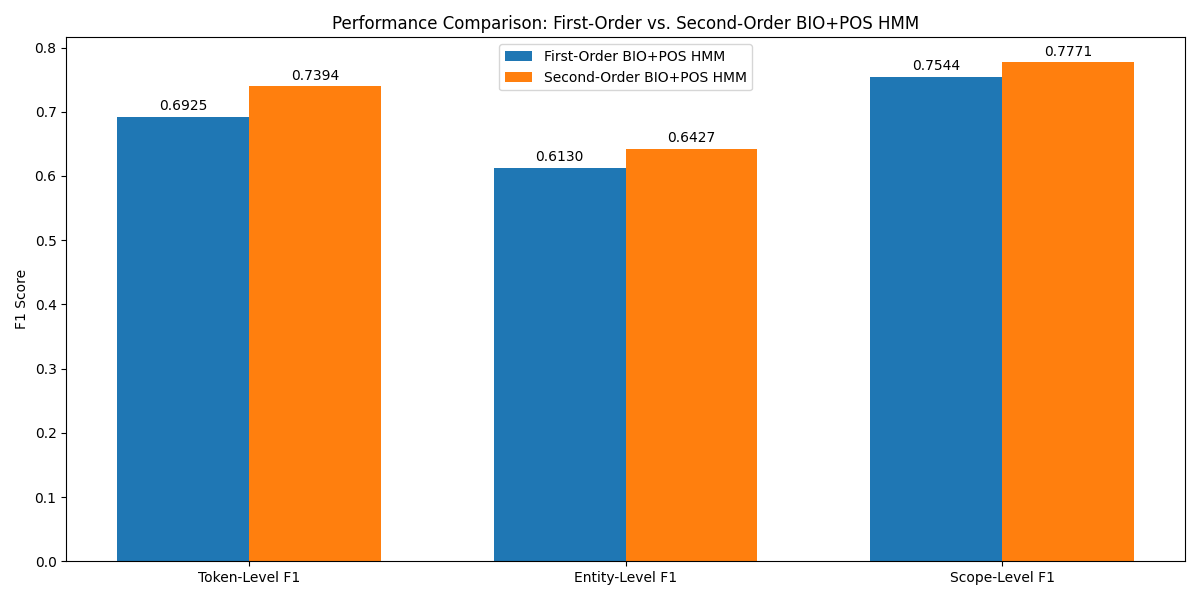
\includegraphics[width=0.90\linewidth]{nlp/figures/first_vs_second_order.png}
            \caption{Performance comparison of our HMM models showing F1 scores at token, entity, and scope levels.}
            \label{fig:hmm-comparison}
        \end{figure}
        
        \begin{table}[h]
        \centering
        \caption{Second-order HMM model classification report with BIO tagging}
        \begin{tabular}{|l|c|c|c|c|}
        \hline
        \textbf{Label} & \textbf{Precision} & \textbf{Recall} & \textbf{F1-Score} & \textbf{Support} \\
        \hline
        NEG (B+I)   & 0.91 & 0.94 & 0.93 & 1152 \\
        UNC (B+I)   & 0.65 & 0.71 & 0.68 & 194  \\
        NSCO (B+I)  & 0.79 & 0.79 & 0.79 & 3273 \\
        USCO (B+I)  & 0.44 & 0.51 & 0.47 & 495  \\
        \hline
        \textbf{Macro Avg}    & 0.73 & 0.76 & 0.74 & 5114 \\
        \textbf{Weighted Avg} & 0.76 & 0.78 & 0.77 & 5114 \\
        \hline
        \end{tabular}
        \end{table}
        
        The second-order model shows significant improvements because it captures longer dependencies between labels. This is especially important for scopes (NSCO, USCO), where context beyond the immediate previous word matters. By using trigram transitions, our model better handles the continuity of scope labels and reduces the error propagation problem that affected the first-order models. As shown in the table, we achieved good results for negation detection, while uncertainty detection remains more challenging.
    \subsection{Error Analysis}
        When we looked at the results more closely, we found that HMMs work well in some cases but not so well in others.
        
        \begin{tcolorbox}[colback=blue!5, colframe=blue!20, sharp corners, boxrule=0.5pt]
        \textbf{Success Case. Simple Negation with Clear Scope}\\
        \textbf{Text.} "actualmente presentan buen aspecto sin signos de sangrado ni infeccion"\\
        \textbf{True labels.} NEG (sin), NSCO (signos, de, sangrado, ni, infeccion)\\
        \textbf{Baseline predictions.} Got both the negation marker and its entire scope right.\\
        \textbf{Analysis.} The baseline HMM handles common patterns like "sin" with a straightforward scope pretty well.
        \end{tcolorbox}
        
        \begin{tcolorbox}[colback=blue!5, colframe=blue!20, sharp corners, boxrule=0.5pt]
        \textbf{Error Case. Uncertainty vs Negation Confusion}\\
        \textbf{Text.} "la motilidad compatible con contractilidad ausente nota no se observa"\\
        \textbf{True labels.} UNC (compatible, con), USCO (contractilidad), NEG (no), NSCO (se, observa)\\
        \textbf{Baseline errors.} Messed up by labeling the uncertainty cue and scope as negation scope (NSCO).\\
        \textbf{Analysis.} The model cannot really tell the difference between uncertainty and negation when they appear close to each other, which shows how limiting it is to only look at the previous state.
        \end{tcolorbox}
        
        All HMM variants struggled with discontinuous scopes and sentences with multiple overlapping expressions. The second-order model performed better on these complex cases, but uncertainty detection remained challenging across all models, with UNC and USCO having lower F1 scores than their negation counterparts.


\addcontentsline{toc}{section}{References}
\printbibliography

%----------------------------------------------------------

\end{document}